\chapter{Technology and Keeping Social Distancing}


\newpage

\begin{center}
\textbf{``Work is what we do, not a place we travel to"}
\end{center}
\begin{figure}[H]
\vspace{-.3cm}
\centering
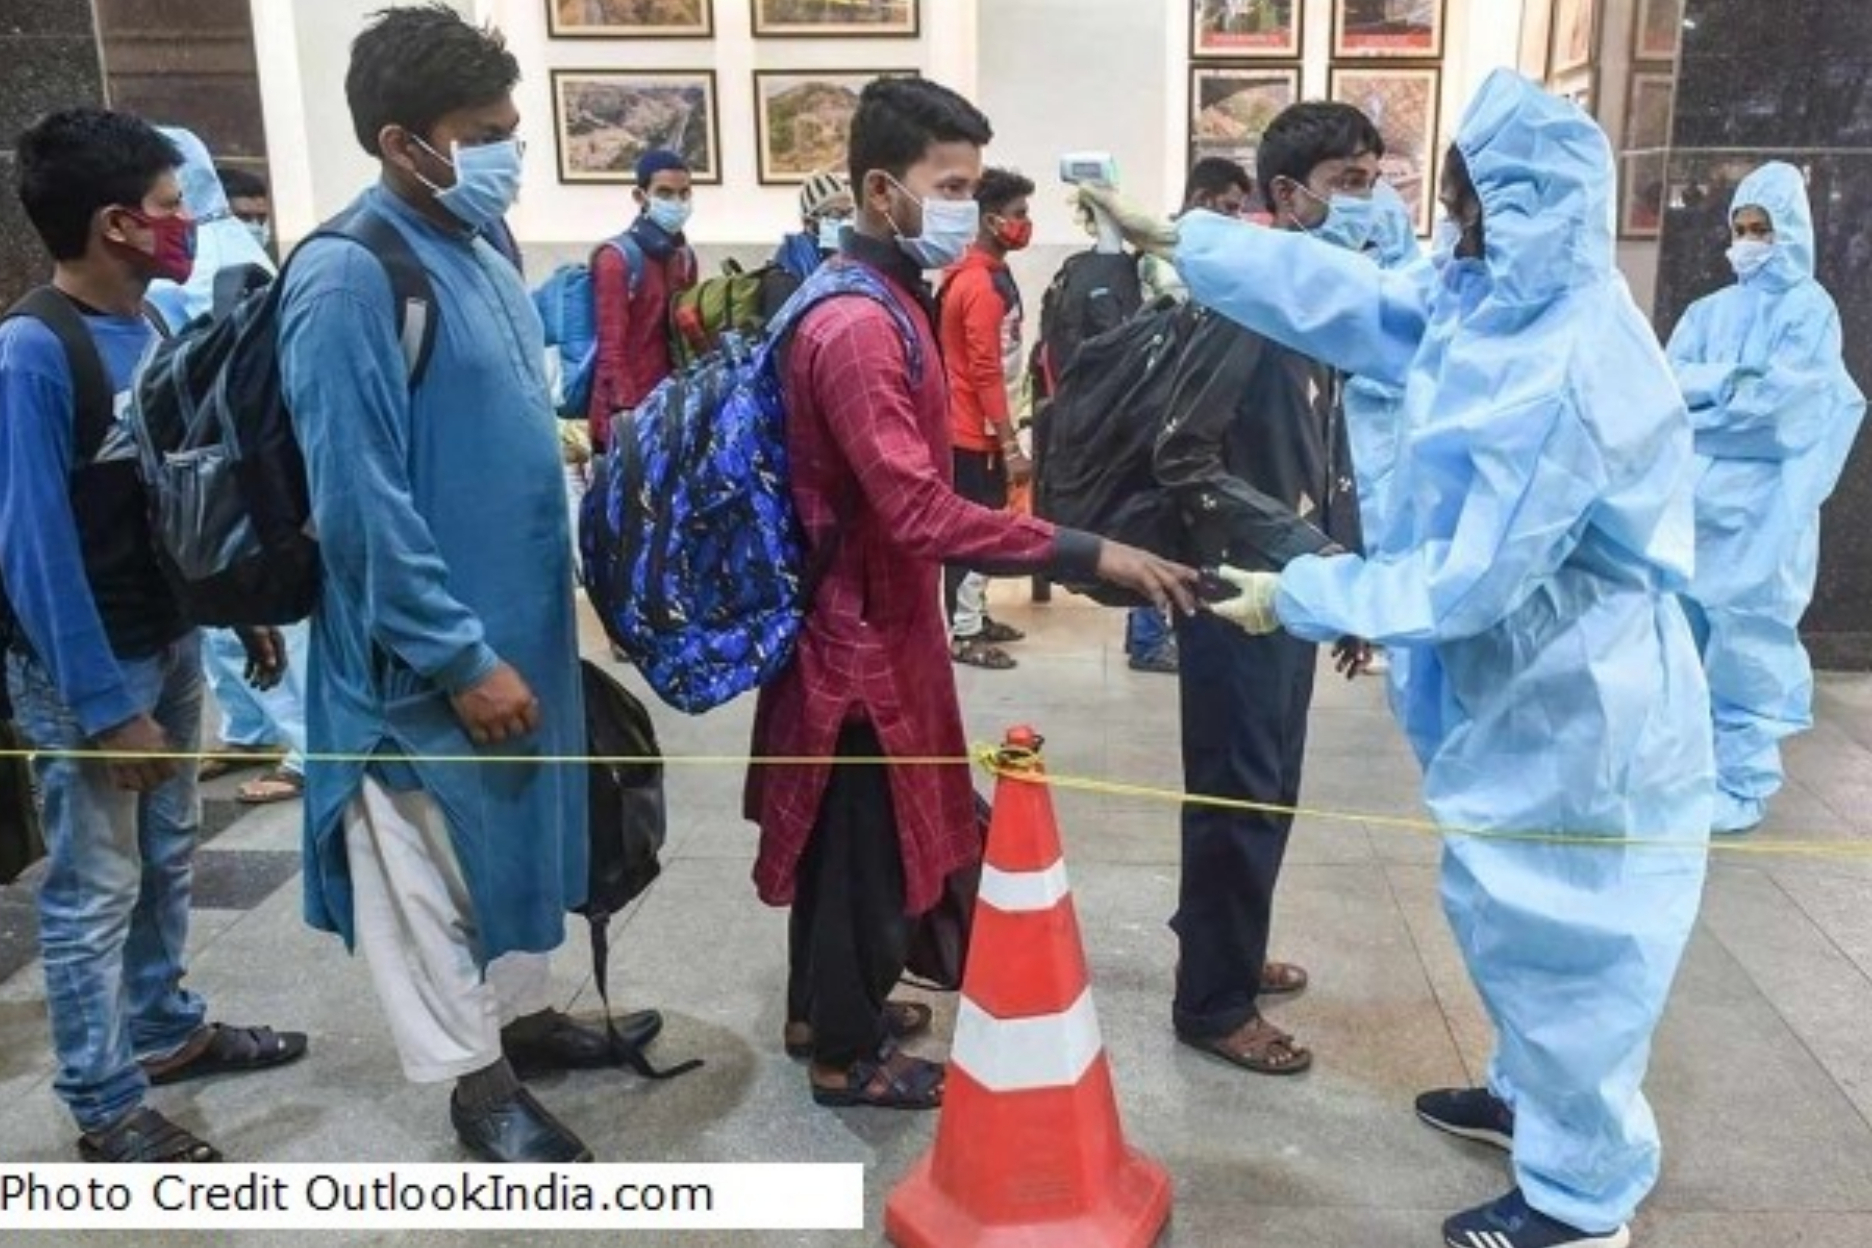
\includegraphics[scale=1.1]{src/Figures/chap3/fig001.jpg}

\end{figure}

\begin{multicols}{2}

\section{The Office Environment}\label{section-1}

\vspace{-.3cm}

The physical environment of office work has changed over the decades. We have all seen images of office workers sitting at tables arranged in rows and columns in some big hall. Officers had their office rooms or cabins. Spending an hour or so to commute to such an office and to spend another hour to commute back in the evening was generally necessary for a large fraction of the employees. The big change that came in the sixties was the introductions of ``cubicles" with separators lower than eye level of a standing person. The separators are usually above the eye level of the sitting employee so that the cubicle gives some feeling of privacy.

Improvements in communication technology, particularly the availability of access to a global Internet, prompted the thought of telework in the seventies \cite{art3-key01}. Anything done away from the traditional workplace is called telework, particularly when a link to the office network and databases is accessible from the place of work. Later, the term telecommuting became a common way of referring to this mode of work. It meant the use of a systematic arrangement whereby the worker avoided the daily commute to the office. 

Why commute when you can do your work from home? Obviously, telecommuting is more suitable for use with employees who are autonomous, have a clear-cut definition of their work, and are very responsible. They do not need constant watching or prodding. It is much easier to adopt telecommuting in white-collar industries than in manufacturing. However, the concept is relevant beyond the context of pure office work. We have not yet seen medical personnel doing much telecommuting, but this is likely to become attractive in the near future. General practitioners are very autonomous, but are now becoming fairly dependent on use of shared facilities for testing, imaging, handling emergencies, inpatient treatment and surgery. This suggests that a doctor could work for a hospital, under their supervision, but at a place convenient to himself and his patients.

\section{Networking individual\\ practitioners}\label{section-2}

Keeping social distancing becomes easier if many employees telecommute. However, they are many other factors that promote telecommuting. Employment in an office or being self-employed at home or at a small, private office have been traditional forms of employment. Optical fibers have vastly improved the bandwidth available to users, making remote work easier. Advances in video technology have made video-conferencing for face-to-face communication or for group communication very affordable. You can access shared information on central computers as easily from your home as from your office.

New forms of employment have created a new form of ``employee", the gig-worker. Gig workers are independent contractors, online platform workers, contract firm workers, on-call workers and temporary workers \cite{art3-key02}. The drivers with Ola and Uber are good examples. A large number of jobs, more or less part-time jobs, have been created by these two companies. They are linked to office computers that manage all customer contact and financial work. Some companies call such contract workers or contract ``partners".

Professionals in a variety of disciplines would benefit from a different arrangement, that of affiliation. Such an affiliation has been seen in the past in the case of insurance agents. Instead of seeking an employer, many professionals could look for a service providing organization. For instance, lawyers, accountants, and dentists could pay a fee to an organization that provides them a variety of services. Lawyers could ask for professional search assistance to look up precedents, court judgements, representation in a court in another city, handling a case for which one lacks expertise, etc. In all cases, affiliation could give the ability to refer one’s patients or clients to a trusted co-worker during a vacation or emergency.

The point is that telecommuting is not a change that stands alone. It is related to a whole variety of ideas changing the nature of work. 

What can engineers do about telecommuting? They face a design challenge. Can they design an office of the future?  A prefabricated enclosure that can be assembled at home to provide a telecommuter a good office environment. It could be equipped with a high bandwidth link to the Internet, one or more large display screens for use with a laptop and for video conferencing. It could have sound proofing and air conditioning. An important item would be software, ideally integrated as an automated secretary or assistant who would use an audio-cum-keyboard input. A ``face-to-face" talk with any one in the office should be possible the moment it is needed. We need to take telecommuting to the next level. 

From the point of view of this article, Telecommuting is one powerful way of social distancing in the context of infectious diseases. We will also discuss other possible solutions to the problem. 

\section{Monitoring of the spread of highly infectious diseases}\label{section-3}

Temperature continues to be an important symptom of many infectious diseases. It is easy to monitor, and it is an early symptom. In a world that is rapidly adopting activity trackers, we should anticipate reliable temperature measurement\footnote{An interesting research question is what makes it difficult for an activity tracker to get accurate measurements of the user’s body temperature. The last one I tried on was off by two degrees centigrade!} to be built into trackers soon. However, utilizing an individual’s temperature to reduce the spread of infectious diseases is not so easy. Social and legal hurdles prevent our requesting every employee in an office to share his temperature information on a daily basis! Imagine the benefits to society if any employee with fever can be expected to, or requested, to stay away from office. In fact, we ought to be able to prevent such persons entering public places like movie theatres, buses, and metros. Yet another possibility is to insist that anyone with a fever should wear a mask anytime they step out of their residence. Once a doctor’s diagnosis is available, the doctor can issue a recommendation on how the precautions can be modified. For instance, if the doctor finds that the fever is due to a non-infectious condition, mask-wearing can be avoided. The doctor should be able achieve this by merely sending a text message to a designated number.

A whole variety of tests can now be carried out by a doctor in a clinic. Lab tests are automated and the results are communicated quickly over the web and email. All this information can be used to minimize the discomfort to the individual with fever and to maximize the protection of the public. 

\vspace{-.3cm}

\section{Keeping the air safe in offices}\label{section-4}

\vspace{-.2cm}

Any office locating a number of workers in an office with its own air circulation system has a responsibility to keep the air free of viruses. Air purifiers with a HEPA\footnote{High Efficiency Particle Absorbing filter. It removes particles as small as 0.3 $\mu$m in size from the air.} filter do trap a large percentage of viruses. Ultraviolet devices incorporated into air purifiers or air conditioners can also provide good protection by actively killing the viruses. An important feature of such active protection against viruses is that it is not specific to one species of virus as vaccines are. They will kill all viruses known, and unknown, as of now.

\newpage

\vspace{-.3cm}

\section{Mode of transmission of viruses}\label{section-5}

\vspace{-.2cm}

Thinking further about keeping office air safe requires that we note some basic facts about how viruses are carried by air. They are not carried as individual particles. To quote a World Health Organization Document \cite{art3-key03}, “Respiratory infections can be transmitted through droplets of different sizes: when the droplet particles are >5-10 $\mu$m in diameter they are referred to as respiratory droplets, and when then are <5$\mu$m in diameter, they are referred to as droplet nuclei. According to current evidence, COVID-19 virus is primarily transmitted between people through respiratory droplets and contact routes. In an analysis of 75,465 COVID-19 cases in China, airborne transmission was not reported.” While the document refers only to Covid-19 viruses, our discussion is relevant to all viruses carried by droplets of the size mentioned. 

In other words, we are dealing with viruses carried by droplet particles larger than 5-10 $\mu$m in diameter. It seems best to treat indoor air being recycled and fresh air taken in from outside the building and sterilize or eliminate infection carrying droplets. The air conditioning units that cool the air vastly increase the number of droplets that don’t need sterilization.

\vspace{-.4cm}

\section{You don’t need to distance yourself from healthy people}\label{section-6}

\vspace{-.2cm}

Many of our problems in handling infectious diseases is that public health services are still working in old-fashioned ways. If you visit a doctor reporting a fever, he is not aware that three persons in your neighborhood tested positive for flu yesterday. We need to network all information such as test reports in a way that patient’s privacy is not violated. Is it not possible to network sharable data like the infectious agent involved, approximate location of the patient without naming him/her? Statistics derived out of such data can indicate to the doctor a likely cause of your fever.

This sharing of infection reports becomes relevant in another context. Suppose the patient who tested positive for flu works in a large office. Should not the information about his flu be made available to a concerned official in his office? The aim should be to ensure that the employee does not attend office for a specified number of days. This is the optimal form of social distancing – it distances the infected from the others! In this case, the individual’s privacy is to some extent compromised. However, suitable practices can be evolved and agreed upon so that the compromise to privacy is minimized. The employer can request cooperation from the employee, particularly if the employer is bearing the cost of medical care.

\begin{thebibliography}{99}

\bibitem{art3-key01} Vicky Gan, The Invention of Telecommuting, Dec 2015, Bloomberg CityLab,


\url{https://www.bloomberg.com/news/articles/2015-12-01/whattelecommuting-looked-like-in-1973}

\bibitem{art3-key02} Katherine Guyot and Isabel V. Sawhill, April 6, 2020 Telecommuting will likely continue long after the pandemic, The Brookings Institution

\url{https://www.brookings.edu/blog/up-front/2020/04/06/telecommuting-will-likely-continue-long-after-the-pandemic/}

\bibitem{art3-key03} Transmission of SARS-CoV-2: implications for infection prevention precautions, Scientific Brief, 9 July 2020 COVID-19: Infection prevention and control / WASH,

\url{https://www.who.int/publications/i/item/modes-of-transmission-ofvirus-causing-covid-19-implications-for-ipc-precautionrecommendations}

\end{thebibliography}

\end{multicols}
